\label{sec:dir_energy_fitting_noise}
%\textit{Smoothing and its empirical evidence for graph classification}
% \begin{figure}
%     \centering
%     % \setcounter{figure}{4} 
    
%     \subfigure[]
%     {
%         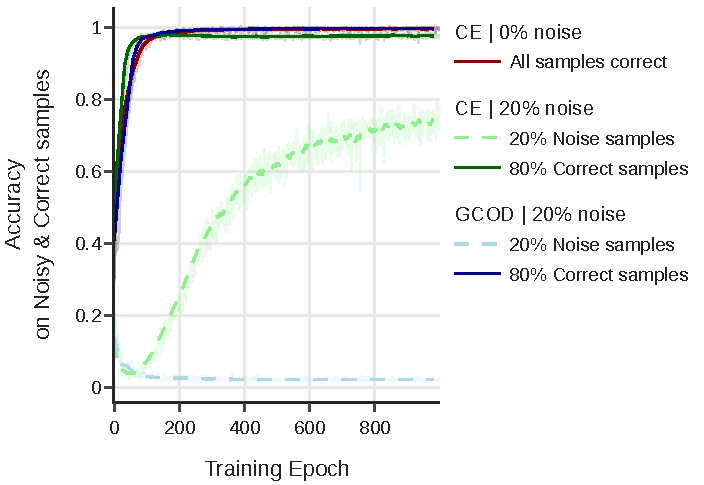
\includegraphics[width=0.47\textwidth]{AISTATS/figures/fig8a}
%         \label{fig:PPA_DE_NCOD_subfig1}
%     }
%     \subfigure[]
%     {
%         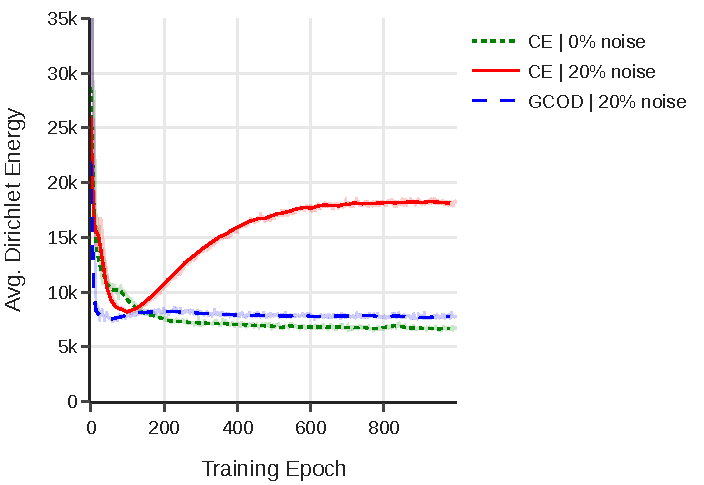
\includegraphics[width=0.47\textwidth]{AISTATS/figures/fig8b}
%         \label{fig:PPA_NCOD_Dirich_energy}
%     }
    
%     % Main figure caption (will still be figure 5)
%     \caption{\ref{fig:PPA_DE_NCOD_subfig1} Avg. training accuracy for GIN model on the PPA dataset (30\% sample, 6 classes) with clean or 20\% label noise. CE represents Cross Entropy, while \method refers to our modified loss function.
%     \ref{fig:PPA_NCOD_Dirich_energy}
% Evolution of Representation Dirichlet energy for clean and noise-introduced PPA dataset (30\% sample, 6 classes). Dirichlet energy increases when the model with CrossEntropy fits on noise.}
%     \label{fig:mainfig}
% \end{figure}
% \begin{figure}
%     \centering
%     % \setcounter{figure}{4} 
    
%     \subfigure[]
%     {
%         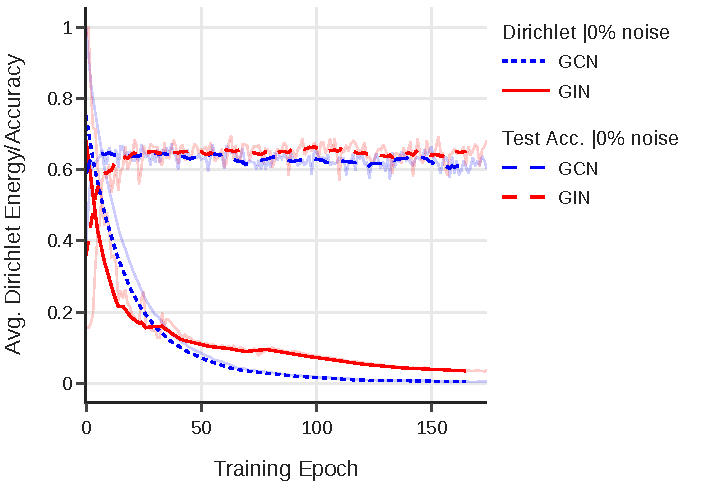
\includegraphics[width=.47\textwidth]{AISTATS/figures/gin_gcn_dir.pdf}
%         \label{fig:gin_gcn_dir}
%     }
%     \subfigure[]
%     {
%         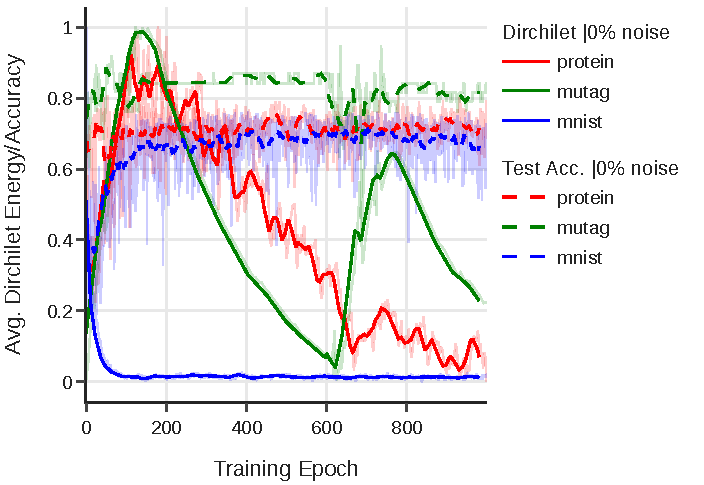
\includegraphics[width=0.47\textwidth]{AISTATS/figures/comapreDataset.pdf}
%         \label{fig:comparedataset}
%     }
%     \caption{\ref{fig:gin_gcn_dir} Evolution of average Dirichlet energy and average test accuracy on the PPA dataset using Cross-Entropy (CE) with GIN and GCN models. 
% \ref{fig:comparedataset}Dirichlet energy and Accuracy evolution on different datasets using GIN model. (Dirichlet Energy is normalized to scale for comparison)}
%     \label{fig:mainfig}
% \end{figure}


\begin{figure}[t]
    \centering

    \subfigure[]
    {
        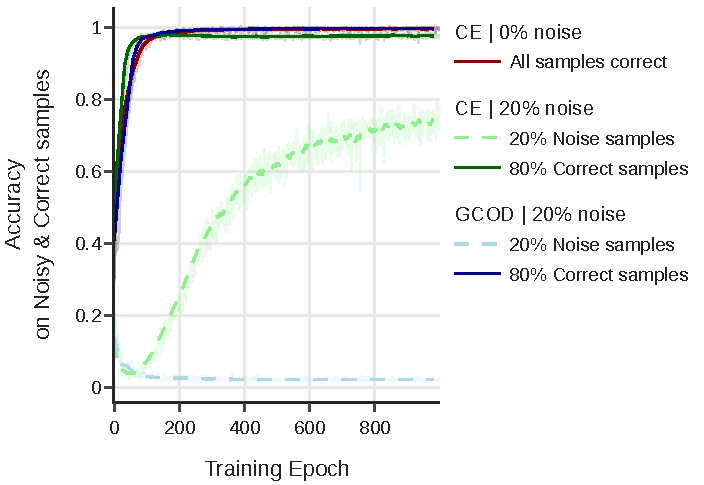
\includegraphics[width=0.47\textwidth]{AISTATS/figures/fig8a}
        \label{fig:PPA_DE_NCOD_subfig1}
    }
    \hfill
    \subfigure[]
    {
        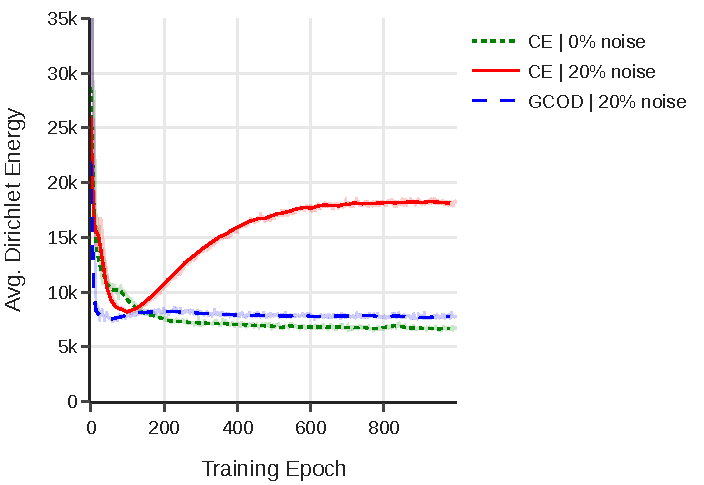
\includegraphics[width=0.47\textwidth]{AISTATS/figures/fig8b}
        \label{fig:PPA_NCOD_Dirich_energy}
    }
    
    \subfigure[]
    {
        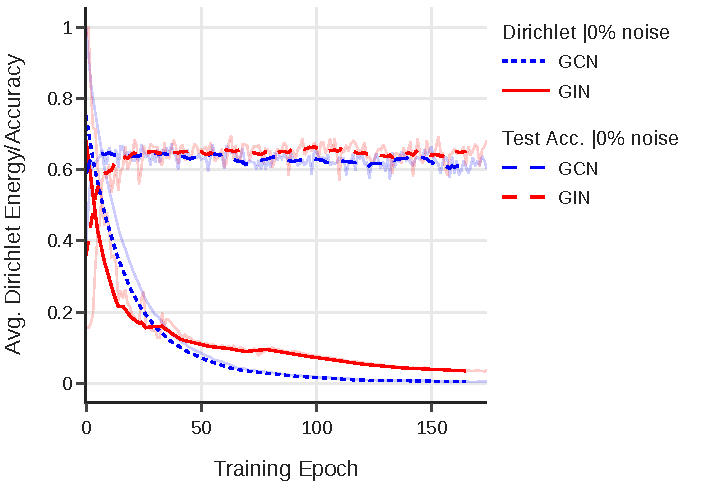
\includegraphics[width=0.47\textwidth]{AISTATS/figures/gin_gcn_dir.pdf}
        \label{fig:gin_gcn_dir}
    }
    \hfill
    \subfigure[]
    {
        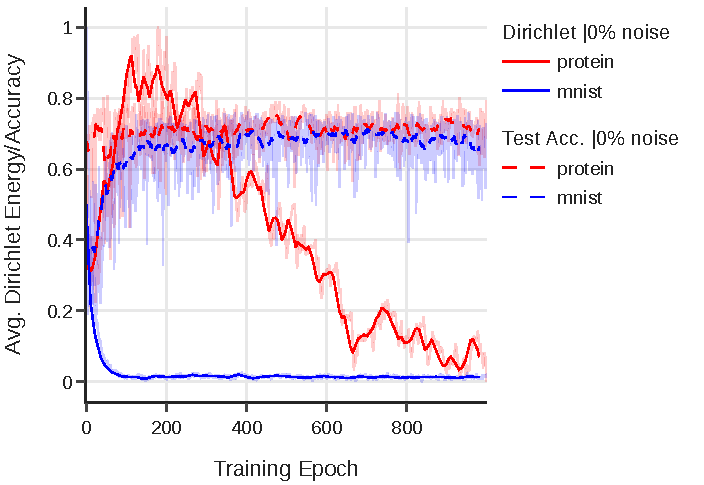
\includegraphics[width=0.47\textwidth]{AISTATS/figures/compareDataset.pdf}
        \label{fig:comparedataset}
    }

    \caption{
    (a) Evolution of training Accuracy for GIN model on the PPA dataset (30\% sample, 6 classes) with clean 0\% or 20\% label noise for CE and \method. 
    (b) Dirichlet energy for clean and noise introduced PPA dataset (30\% sample, 6 classes). The Dirichlet energy increases when the model with CE fits on noise.
    (c) Dirichlet energy and test Accuracy on the PPA dataset using CE with GIN and GCN models.
    (d) Dirichlet energy and test Accuracy on different datasets using GIN model (axes scaled for comparison).
    }
    
    \label{fig:dirichlet_results}
\end{figure}

% Crucially, behavior differs on a dataset with noise. After the initial training phase, the model fits on noisy samples (observe an increase in training accuracy on noisy samples for CE-20\% in Fig. \ref{fig:PPA_DE_NCOD_subfig1}). Notice, that the fitting on noise is accompanied by a significant increase in Dirichlet energy $E^{dir}_{\text{set}}(\mathcal{D}_c)$ (see CE-20\% in Fig. \ref{fig:PPA_NCOD_Dirich_energy}). 

Across all experimental setups, we consistently observe that the Dirichlet energy (\(E^{\text{dir}}\)) of the learned node representations increases once the model begins to fit on noisy labels (see Fig. \ref{fig:PPA_NCOD_Dirich_energy}). During early training, when the model captures true patterns, \(E_{\text{dir}}\) remains low; however, as the model starts fitting the noisy samples, the energy increases significantly. This consistent behavior across diverse datasets and conditions ( Fig. \ref{fig:PPA_NCOD_Dirich_energy} 
 and Figure \ref{fig:dirichlet_energy_comparison})  motivates us to use \(E^{\text{dir}}\) as a signal to detect and monitor overfitting to label noise.

%This empirical observation aligns with theoretical understanding of GNNs. The learnable weight matrices in GNN layers determine whether features are smoothed across the graph  or sharpened. Sharpening directly increases the Dirichlet energy \cite{zhou2021dirichlet}.
%We conjecture that training on noisy labels, especially those creating false distinctions between similar graphs, forces the model to amplify high-frequency differences to fit these contradictory signals. This process increases the signal's high-frequency content and Dirichlet energy, enabling the model to fit the noise.

This leads to our first research question \textbf{RQ1}:\textit{ Is Dirichlet energy related to GNN performance on graph classification tasks, and how does it evolve when label noise is introduced during training?} 

To address this, we propose a graph-level Dirichlet energy measure for the graph classification task and analyze its empirical behavior during training under noise conditions.
Given a set of graphs $\mathcal{S}$, composed of graphs $\mathcal{G}^i$ with latent representation $\mathbf{Z}^i$, we define the Dirichlet energy of the set $\mathcal{S}$ as
\begin{equation}
    \label{eq: avg_dirichlet}
   E^{dir}_{\text{set}}(\mathcal{S}) := \frac{1}{|\mathcal{S}|} \sum_{\mathcal{G}^i \in \mathcal{S}}  E^{dir}(\mathbf{Z}^i).
\end{equation}


In particular, we study $E^{dir}_\text{set}(\mathcal{D}_c)$, the average Dirichlet energy of graphs belonging to class $c$, where $\mathcal{D}_c$ denotes the subset of training graphs with the label $c$. 


Our empirical analysis provides a consistent answer to \textbf{RQ1}. In clean datasets, i.e., without label noise, \( E^{dir}_{\text{set}}(\mathcal{D}_c) \) may fluctuate during the initial training phase as the model begins to adjust to the task. However, we consistently observe a steady decrease in the later stages of training, culminating in low and stable Dirichlet energy values once the model converges to high classification accuracy. This behavior is illustrated in Fig.~\ref{fig:gin_gcn_dir} and Fig. \ref{fig:comparedataset} for models trained with standard Cross-Entropy (CE) loss and no label noise (CE-0\%).

However, when synthetic label noise is introduced (e.g., 20\% symmetric flipping), the behavior diverges. As shown in Fig.~\ref{fig:PPA_DE_NCOD_subfig1}, while the initial phase of training still exhibits a decrease in \( E^{dir}_{\text{set}}(\mathcal{D}_c) \), this is followed by a significant increase during later epochs, precisely when the model starts to fit the noisy labels. This memorization phase is marked by rising training accuracy on noisy samples (see CE-20\%), demonstrating a direct link between noise fitting and increased Dirichlet energy.
This phenomenon is consistently observed across datasets and model architectures, including MUTAG, MNIST, and PROTEINS (see 
Fig. \ref{fig:comparedataset} and Fig. \ref{fig:mutag} in Appendix \ref{appendix:additional_figures}). These findings confirm that Dirichlet energy serves as a reliable signal of representation smoothness and its disruption as a result of noise memorization.

Furthermore, to isolate the spectral dynamics, we utilize the HLFF-GNN framework \citet{hlffgnn}, which decomposes the node representations into low-frequency \( \mathbf{Z}_1 \) and high-frequency \( \mathbf{Z}_2 \) components. Experiments show that while \( E^{dir}(\mathbf{Z}_1) \) remains stable, \( E^{dir}(\mathbf{Z}_2) \) sharply increases during noise overfitting, confirming that high frequency energy components are responsible for fitting mislabeled data (detailed analysis of these experiments is provided in Appendix \ref{sec:Amplification}).

From these observations, we conclude that maintaining a low Dirichlet energy, particularly by suppressing some high-frequency components, correlates with robust generalization. However, directly minimizing \( E^{dir}_{\text{set}}(\mathcal{S}) \) as a loss term presents practical challenges. First, the asymptotic energy level varies between datasets and architectures, making it difficult to define a universal target. Second, \( E^{dir}_{\text{set}} \) is a global dataset level quantity, which is not easily decomposed into sample gradients for stochastic optimization. We propose alternative strategies to promote smoothness. 
% Therefore, rather than optimizing \( E^{dir}_{\text{set}} \) directly, we propose alternative strategies to promote smoothness indirectly. 
% In the next section, we introduce two such methods: (1) a spectral regularization scheme that alters GNN propagation to favor low-frequency outputs, and (2) a modified loss function (GCOD) that incorporates a smoothness-aware correction signal. These methods are designed to preserve the natural smoothing bias of GNNs while enhancing robustness to noisy supervision.

% Our empirical results confirm \textbf{RQ1} hypothesis, showing a strong relation between the model improving performance and decline of $E^{dir}_\text{set}(\mathcal{D}_c)$. During the initial learning phase, for all models and noise mixtures, we observe $E^{dir}_\text{set}(\mathcal{D}_c)$ declines. 

% For the datasets without noise, upon reaching stable accuracy indicative of convergence, the $E^{dir}_\text{set}(\mathcal{D}_c)$ also attains its minimum and reaches an asymptotic stability (see models trained using Cross-Entropy (CE) loss function on a training set without noise "CE-0\%" in Fig. \ref{fig:gin_gcn_dir}). 


% Thus, when the model learns samples outside of each class distribution (noisy, mislabelled samples), the overall node representation smoothness in a class decreases, which is confirmed by the increase in  $E^{dir}_\text{set}(\mathcal{D}_c)$. This finding underscores the critical importance of understanding smoothness for graph classification. Thus, we conclude that enhancing smoothness should increase the model's robustness to noise and improve performance. 

% No results - commenting out
%To further validate this hypothesis, we conducted tests using the synthetically generated dataset described in Section \ref{sec:experimental_setting}.

% This behavior was consistent even in other datasets with similar training configurations, such as MUTAG, MNIST, and PROTEINS, see Fig. \ref{fig:comparedataset} in Appendix \ref{appendix:additional_figures}. 
%  In our subsequent experiments, we employed the same settings but introduced 20\% noisy labeled samples into the dataset to reevaluate the outcomes. We did not observe a significant deviation from the previously observed trend of accuracy and $E^{dir}(\mathcal{D}_c)$. Notably, $E^{dir}(\mathcal{D}_c)$ followed a similar trajectory, showing a significant decrease and corresponding with improved classification accuracy. However, the overall $E^{dir}(\mathcal{D}_c)$ values were higher at every instance compared to the non-noisy scenario, yet the trend remained consistently decreasing, see Figure \ref{}. \textcolor{red}{NO FIGURE, REMOVE?}) This behavior was somewhat unexpected as there was no substantial drop in accuracy despite the inclusion of noisy samples in the dataset. To further investigate this phenomenon, we plotted the training accuracies on both pure and noisy samples. The results indicated that the model either did not fit the noise completely or did so only insignificantly, which explains the continued decline of $E^{dir}(\mathcal{D}_c)$.



% REMOVING - ALREADY EXPLAINED ABOVE, MOSTLY DUPLICATE
%Our analysis of the non-noisy dataset revealed a consistent trend in the behavior of $E^{dir}(\mathcal{D}_c)$, albeit with reduced magnitudes as training progressed. The experiments showed that the decrease in Dirichlet energy corresponded to an overall increase in classification accuracy, maintaining the observed trends.
%Further experimentation with the reintroduction of 20\% noisy samples revealed a critical insight: the model's tendency to fit noisy samples was accompanied by an increase in the $E^{dir}(\mathcal{D}_c)$ of the graphs. Thus, when the model fits on noisy data, it increases the overall $E^{dir}(\mathcal{D}_c)$ of the class, indicating a reduction in smoothness, see Figure \ref{fig:mainfig}. This finding underscores the critical importance of smoothness for graph classification. Therefore, any approach that enhances smoothness should either improve accuracy or render the model more robust to noise. To further validate this hypothesis, we conducted tests using the synthetically generated dataset described in Section \ref{sec:experimental_setting}.

%All the experiments described so far were performed using a model based on GIN layers. Extending our analysis to other message-passing rules like GCN models, we observed similar trends, for further details see the section in the Appendix \ref{}. We conducted similar experiments on the MNIST and Enzyme datasets, observing comparable trends, results are reported in Section \ref{} in the Appendix. The MNIST results closely followed the expected profile, while the Enzyme dataset showed slight deviations, likely due to its smaller size of 600 graphs.




%\subsection{Limitations of using Dirichlet Energy as a loss target}
% Given these observations, the natural follow-up question is whether we can directly optimize for the reduction of Dirichlet Energy to make a GNN model robust. We find such an approach quite challenging, thus we need alternative methods that incentivize smoothness captured by Dirichlet Energy. Specifically, we observed that the asymptotically suitable  value of Dirichlet Energy is always above 0, and reaches a value specific to each dataset and model, which makes it hard to generalize. Secondly, Dirichlet Energy by definition requires overall dataset optimization, which requires proxies to decompose into sample-level loss functions. Therefore, next, we offer two different methods to enforce smoothness.
% through training and loss modifications.
% \begin{figure}[t!]
%     \centering
%     \begin{subfigure}[b]{0.5\textwidth}
%         \centering
%         %\includegraphics[scale = 0.25]{Neurips/Screenshots/gin_drchi_6Classes_30/20_N_P_drichi.png}
%         %
\includegraphics[page=1,width=1.0\textwidth]{Neurips/figures/fig8a}
%         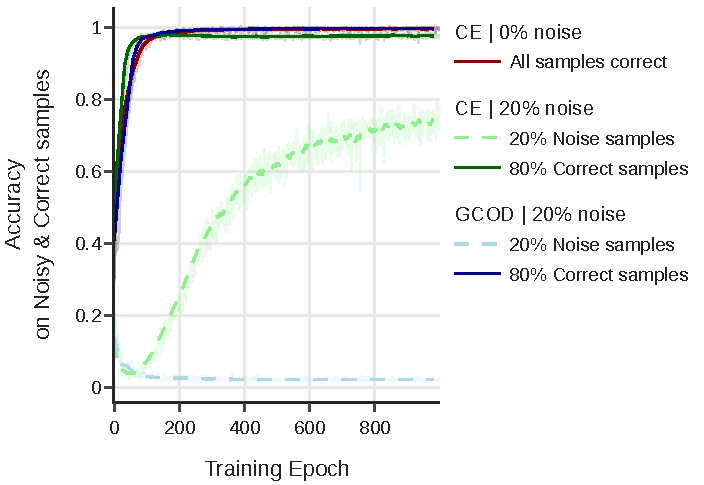
\includegraphics[page=1,width=1.0\textwidth]{AISTATS/figures/fig8a}
%         \caption{Avg. Accuracy for GIN model on the PPA dataset (30\% sample, 6 classes) with clean or 20\% label noise. CE represents Cross Entropy, while \method refers to our modified loss function. 
%         %In particular, we show the average accuracy for three classes ( taken from the 6). For the case with 0\% noise, there are no noisy samples and we reported the accuracy of all samples. For the case of 20\% noise, we reported both the average accuracy of pure samples and the average accuracy of noisy samples.  
%         }
%         \label{fig:PPA_DE_NCOD_subfig1}
%     \end{subfigure}
      
%     \begin{subfigure}[b]{0.5\textwidth}
%  \centering
%         %\includegraphics[scale = 0.25]{Neurips/Screenshots/gin_drchi_6Classes_30/differntnoise_Dirchi_CE_NCOD.png}
%         %
\includegraphics[page=1,width=1.0\textwidth]{Neurips/figures/fig8b}
%         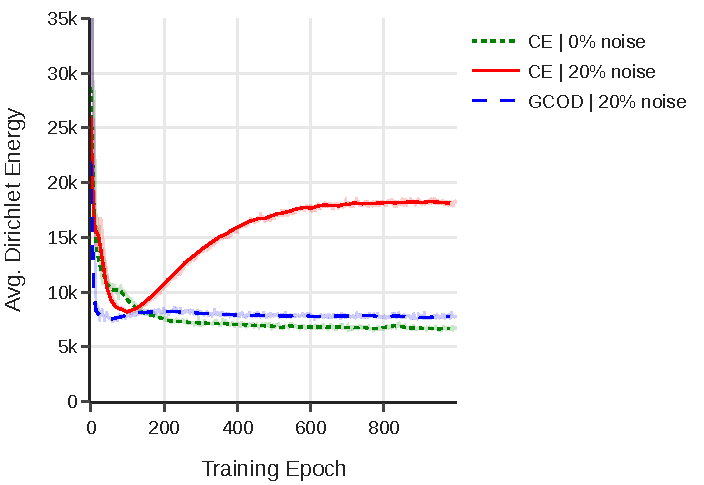
\includegraphics[width=\textwidth]{AISTATS/figures/fig8b}
%         \caption{Evolution of Representation Dirichlet energy for clean and noise-introduced PPA dataset (30\% sample, 6 classes). Dirichlet energy increases, when the model with CrossEntropy fits on noise. }
%         \label{fig:PPA_NCOD_Dirich_energy}
%     \end{subfigure}
%     \caption{}
%     % \caption{Illustrates the evolution of both energy and accuracy throughout the training process}
%     \label{fig:mainfig}
% \end{figure}
% s, can we just include it in the loss function to prevent fitting on problematic samples? Extra work would be required since we cannot include Dirichlet Energy in the loss function directly, because:
%  \begin{itemize}
%      \item DE should approach 0, but not become 0 when no difference between samples is observed. Cannot be directly optimized for
%      \item We cannot offer yet the best target value for DE, which is specific to each task
%      \item? Loss will have to become more complex, comparing pairs or sets of samples (not sure about this, need to think through)
%      \item?
%  \end{itemize}






